\documentclass{beamer}
\input{flat-blue-theme.inc}
\input{footnotes.inc}

\usepackage[T1]{fontenc}
\usepackage[utf8]{inputenc}
\usepackage[ngerman,english]{babel}
\usepackage[english]{datetime2}

\usepackage{tikz}

%
% BibTex
%

% Must be placed here before BibTeX and URL/ref related packages:
\PassOptionsToPackage{obeyspaces}{url} % Allow spaces in URLs
\PassOptionsToPackage{spaces}{url}     % Enable line breaks in URLs

\usepackage[toc, page]{appendix}
\usepackage[
	backend=bibtex8,
	style=numeric,
	sorting=none,
	urldate=long,
	backref
]{biblatex}
\usepackage{hyperref}
\usepackage[noabbrev]{cleveref}

\addbibresource{sources.bib}
\let\oldCite\cite
\renewcommand{\cite}[2][]{ \oldCite[#1]{#2}} % Add space before citation

\NewBibliographyString{diplomathesis}
\DefineBibliographyStrings{english}{
	diplomathesis = {diploma thesis},
}

%
% Commands
%

\newcommand{\bigo}[1]{\mathcal{O}(#1)}

% Environment to center content of a figure without adding extra spacing before the caption
\newenvironment{figcenter}
{%
	\parskip=0pt%
	\par%
	\nopagebreak%
	\centering%
}%
{%
	\par%
	\noindent%
	\ignorespacesafterend%
}

%
% Styling, Layout
%

\setbeamercovered{invisible}
\beamertemplatenavigationsymbolsempty
\condensedToc

% Remove subsection bar
\defbeamertemplate*{headline}{miniframes theme no subsection}
{%
	\begin{beamercolorbox}[colsep=1.5pt]{upper separation line head}
	\end{beamercolorbox}
	\begin{beamercolorbox}{section in head/foot}
		\vskip2pt\insertnavigation{\paperwidth}\vskip4pt
	\end{beamercolorbox}%
	\begin{beamercolorbox}[colsep=1.5pt]{lower separation line head}
	\end{beamercolorbox}
}

%
% Metadata
%

\title[Master's thesis -- Colloquium]{A Hybrid Algorithm for Finding Shortest Paths Between Arbitrary Coordinates using a Combination of Network and Geometric Routing}
\author{Hauke Stieler}
\institute[Universität Hamburg -- Databases and Information Systems]{
	Universität Hamburg\\
	Faculty of Mathematics, Informatics and Natural Sciences\\
	Department of Informatics\\
	Databases and Information Systems
}
\date{\today}
\titlegraphic{
\includegraphics[width=0.3\textwidth]{../thesis/images/UHH-Logo_2010_Farbe_CMYK.pdf}}

\begin{document}
	{
		\setbeamertemplate{headline}{}
		\setbeamertemplate{footline}{}
		\vspace*{-0.8cm}
		\maketitle
		\addtocounter{page}{-1}
	}
	
	\begin{frame}[t]{Inhalt}
		\tableofcontents[hidesubsections]
	\end{frame}
	
	\section{Motivation}
	
		\begin{frame}{Realistic pedestrian routing}
			Beneficial for
			\begin{itemize}
				\item real-world end-user applications\\\textrightarrow\ indoor navigation, campus navigation
				\pause
				\item higher level applications\\\textrightarrow\ isochrones, walkability analysis
				\pause
				\item \textbf{agent-based simulations}\\\textrightarrow\ crowd behavior in evacuation scenario
			\end{itemize}
		\end{frame}
	
		\begin{frame}{Routing techniques}
			Graph-based:
			\begin{itemize}
				\item graph with edges representing roads / ways
				\item well optimized: Dijkstra, A*, speedup techniques
				\item detailed attributes in edges
				\pause
				\item only vertices are reachable\ \textrightarrow\ unable to traverse open spaces
			\end{itemize}
			\pause
			\vspace{2ex}
			Geometric routing:
			\begin{itemize}
				\item shortest path in presence of obstacles (i.e. lines and polygons)
				\item two strategies:
				\begin{itemize}
					\item graph generation (e.g. visibility graphs) + graph-based routing
					\item continuous Dijkstra
				\end{itemize}
				\pause
				\item path realism heavily depends on data quality
			\end{itemize}
		\end{frame}
	
		\begin{frame}{Example 1: Pure graph-based routing}
			\begin{figure}[t]
				\begin{figcenter}
					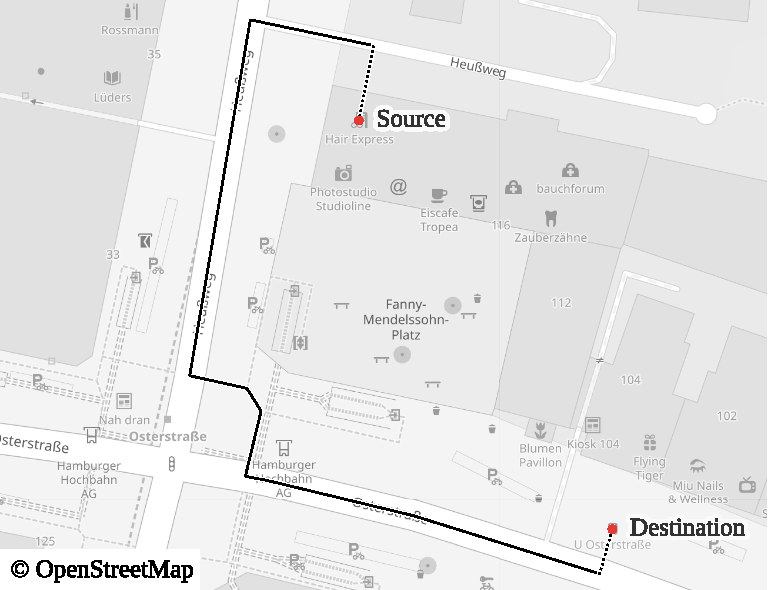
\includegraphics[width=0.5\textwidth]{images/qgis-routing-osterstrasse_routing.pdf}
				\end{figcenter}
				\caption{Graph-based routing result using \href{https://www.osm.org/directions?engine=graphhopper\_foot\&route=53.57657,9.95210;53.57601,9.95268}{\emph{GraphHopper}}.}
			\end{figure}
		\end{frame}
		
		\begin{frame}{Example 1: Expected routing behavior}
			\begin{figure}[t]
				\begin{figcenter}
					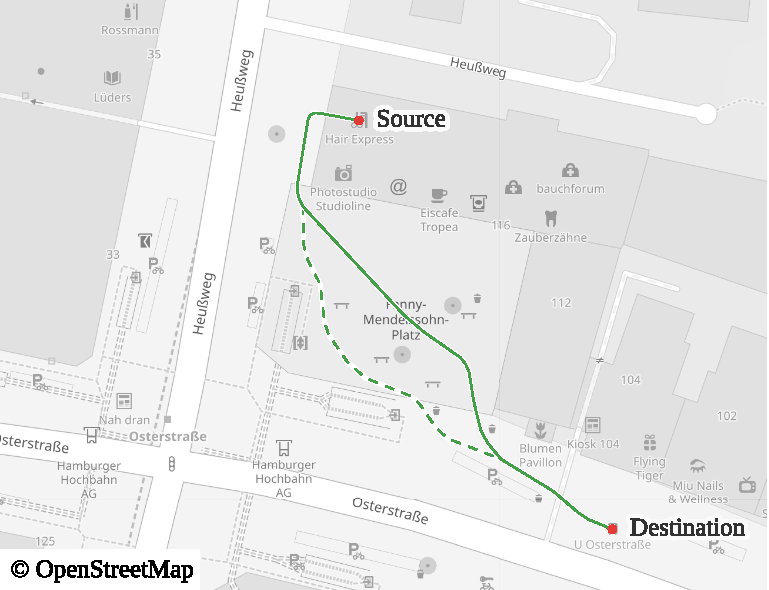
\includegraphics[width=0.5\textwidth]{images/qgis-routing-osterstrasse_expected.pdf}
				\end{figcenter}
				\caption{Routes an actual pedestrian would likely choose.}
			\end{figure}
		\end{frame}
		
%		\begin{frame}{Example 2: Densely built-up areas}
%			\begin{figure}[t]
%				\begin{figcenter}
%					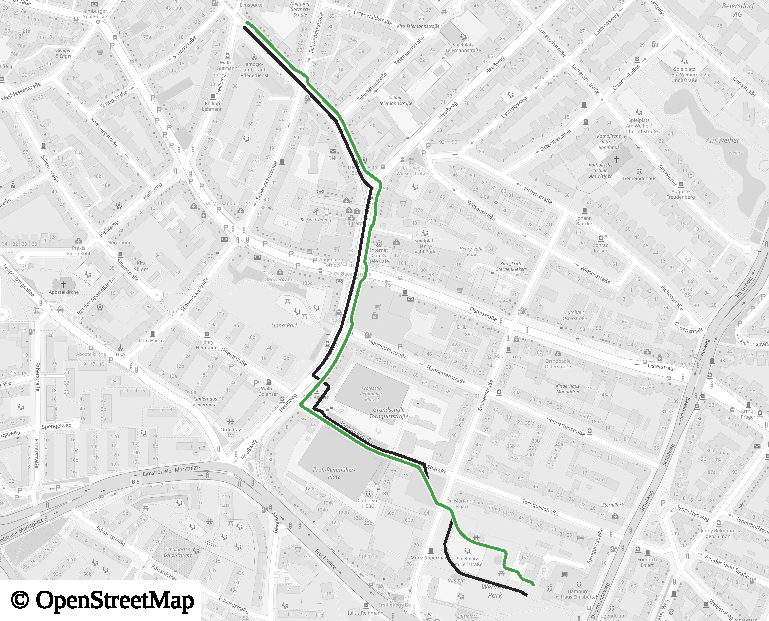
\includegraphics[width=0.5\textwidth]{images/qgis-routing-similar.pdf}
%				\end{figcenter}
%				\caption{Expected routes often follow graph edges, which hold valuable information.}
%			\end{figure}
%		\end{frame}
		
		\begin{frame}{Value of graph data}
			Graph data is still valuable:\n
			\begin{itemize}
				\item detailed information
				\begin{itemize}
					\item surface conditions, access restrictions, allowed vehicle types
				\end{itemize}
				\item definitely walkable
				\begin{itemize}
					\item no real-world obstacles in the way
				\end{itemize}
				\item sometimes without alternatives
				\begin{itemize}
					\item bridges, tunnels
					\item paths through obstacles (e.g. building passages)
				\end{itemize}
			\end{itemize}
		\end{frame}
		
		\begin{frame}{Wanted routing algorithm}
			Should be able to\n
			\begin{itemize}
				\item traverse open spaces
				\item use roads and ways
				\item reach arbitrary locations
				\item create more realistic routes than purely graph-based routing
			\end{itemize}
		\end{frame}
	
	\section{Design}
	
	\section{Implementation}
	
	\section{Evaluation}
	
	\section{Conclusion}
\end{document}